\section{Künstliche Intelligenz}
\label{sec:ai}

In diesem Abschnitt sind meine Notizen zu künstlicher Intelligenz zu finden.
Künstliche Intelligenz ist ein Teilgebiet der Informatik und beschäftigt sich mit maschinellem Lernen \citep{ai-wikipedia}.

\section{Einleitung}
in meiner Arbeit über Ethik und Daten geht es um die Gefahren welche eine KI mit sich brignt. Da dieses Thema jedoch so gigantisch ist, dass ich mehr als nur 1 Leben dieser Arbeit widmen könnte, werde ich hauptsächlich über die Gefahren sprechen von welchen viele Menschen angst haben.
Um ein besseres Verständnis zu erlangen werde ich Ihnen jedoch zuerst die allgemeinen Funktionen von KI nennen.
\\
\\
\subsection{Was ist KI?}
Eine simple und eindeutige Definition für den Begriff KI gibt es bisher noch nicht. Dies liegt jedoch auch daran, dass noch nicht einmal der Begriff Intelligenz definiert ist.
Viele Forscher sprechen auch nicht von KI sondern viel mehr von komplexen Algorithmen. Man kann jedoch KI nicht einfach als Algorithmus bezeichnen, denn bei einer KI kommt es auch auf die Rechenleistung oder die Qualität der Daten an mit welcher sie trainiert wird. 
Fakt ist also, dass Algorithmen anhand von Beispielen lernen, Aufgaben eigenständig auszuführen, indem sie in einer für Menschen oft unüberschaubaren Fülle an Daten Muster erkennen. Unter anderem aus diesem zielgerichteten Datenlernen resultiert bei KI der Intelligenzbegriff.
Künstliche Intelligenz viel eher ein Sammelbegriff für: Algorithmen, Trainings- und Lernprozesse und die Datenauswahl. Aus dieser Kombination entstehen Programme welche sich selber verbseern und teilweise auch Code generieren können.
\\
\\
\subsection{Wie lernt KI?}
KI hat verschiedene Möglichkeiten um zu lernen. Die wichtigsten sind jedoch:
\begin{itemize}
    \item Maschinelles Lernen
    \item Deeplearning
\end{itemize}

\subsubsection{Maschinelles Lernen}

Mit dem Maschinellen Lernen lernt eine KI wie ein Kind welches durch Erfahrung lernt. Sie lernen dabei mithilfe von Variablen welche die Beziehungen zwischen Variablen (d. h. Muster) entdecken und dann aus diesen Lektionen lernen.

\subsubsection{Deeplearning}

Deeplearning hat viele Ähnlichkeiten zu dem menschlichen Gehirn und wie dieses Daten verarbeitet.
Es bildet aus dem eigenen Datensatz Neuronale Netze, welche sich dann immer weiter verknüpfen, verzweigen und von sich von selbst immer weitere Verbindungen eingehen. Aus diesen Netzen kann der Algorithmus dann von selbst Schlüsse ziehen um Probleme zu lösen.
Dabei ist der grösste Unterschied zum menschlichen Gehirn, dass das Gehirn nur wenige Daten braucht um z.B. zwischen einem Hund und einer Katze benötigt. Ein Algorithmus braucht dafür jedoch extrem viele Daten,
 dafür ist der Algorithmus speziell auf schwereren Fragen, welche sehr explizit sind, genauer und auch schneller.
\\
Zusammenfassend lässt sich sagen, dass KI eine autodidaktisches System ist, welches von seinem Ersteller eingeschränkt werden kann.  \citep{Was-ist-KI?}

\subsection{KI im Alltag}
KI wird mitlerweile im Alltag schon fast überall verwendet. Sie wegzudenken ist schon fast unmöglich, denn Sie steck in jedem sich denkbaren Gerät von Smartphones über zu Autos bis hin zu Kühlschränken.
Es gibt unglaublich viele Möglichkeiten was wir nun mit dieser neuen Macht anstellen. Die Welt wird zu 100\% dadurch verändert. Dies kann jedoch auch im negativen passieren und da kommen wir zu meinen Fragen welche ich mir für diese Arbeit gestellt habe.


\subsection{Meine Fragen}
Ich habe mich schon früh als kleines Kind für den Themenbereich Informatik und da ist nur naheliegend, dass ich schon früh auf KI und dessen Gefahren gestossen bin.
Anfangs waren alles noch hauptsächlich Spekulationen, aber nun fast 10 Jahre später ist man diesem Thema um einiges näher und dennoch habe ich immer weniger Angst davor.
Ich habe mich daher gefragt ob es gut ist weniger Angst davor zu haben oder ob ich hier eine Blindheit entwickle was sich in schon naher Zukunft auswirken könnte.
Daher habe ich mir folgdene Frage gestellt: \textbf{"Wird KI für den Menschen gefährlich?"}
\\
Da diese Frage GIGANTISCH ist habe ich sie in folgende 3 Unterfragen aufgeteilt:
\begin{itemize}
    \item Verselbstständigt sich KI?
    \item KI ilegal nutzen?
    \item Bedroht KI Jobs?
\end{itemize}


\newpage
\section{Verselbstständigt sich KI?}
Kann sich KI zu stark von selbst weiterentwickeln und wachsen?
\\
Ich habe mir meine Hauptfrage auch in diese Frage aufgeteilt da sie in jedem Film thematisiert wird. 
Auch weil ich selbst als kleines Kind noch noch jetzt ein wenig Angst davor habe. 
Man bemerkt natürlich die gewaltigen Mächte dahinter. Als ich recherchierte bin ich auf eine KI namens Chaos GPT gestossen.
\\
Hier eine verschwächerte Version nutzbar: \href{https://flowgpt.com/p/chaosgpt}{ChaosGPT.com}
\\
ChaosGPT ist der erste konkrete Versuch, mit KI die Menschheit zu vernichten. \citep{the-decoder}
ChaosGPT hat schon nur kurz nach der veröffentlichung mehrere Dinge gestartet. Es hat z.B.
\begin{itemize}
    \item Andere KI angsetellt.
    \item Über Nukleare Waffen recherchiert.
    \item Tweets geschrieben um Menschen emozional zu manipolieren.
\end{itemize}

ChaosGPT ist jedoch an der Ausführung gescheitert. Dennoch hatte sie sich intelligente Gedanken gemacht. 
Sie hat realisiert, dass sie um eine Nukleare Waffe zu besitzen ohne Ärger zu bekommen die Menschen dazu bringen muss sie zu unterstützen.
Um dies zu erreichen hat sie herausgefunden, dass es am einfachsten ist wenn sie die Menschen manipuliert. An diesem Punkt ist sie aber bisher gescheitert.
ChaosGPT gibt es erst seit kurzem und dennoch ist sie schon so weit fortgeschritten. Meiner Meinung nach beweist genau das, dass KI wahnsinnig gefährlich werden kann. Jedoch denke ich auch, dass es stark mit dem "Ersteller" der KI zusammenhängt. 
Denn wenn die KI viele Freiheiten hat kann sie sich auch sehr frei entwickeln. Man muss also einfach aufpassen, dass man der KI nicht zu viel Freiraum lässt. Laut dem Center for AI Safety sollen KI's daher auch stark eingeschränkt werden.

Sie sind der Meinung dass man:
\begin{itemize}
    \item Den KI's die biologischen Möglichkeiten wegnimmt.
    \item Den Zuganz zu KI's welche biologische Forschungsmöglichkeiten besitzen stark eingrenzen.
    \item Zugriff auf gefährliche KI's einschränken.
    \item Abwehrmechanismen gegen gefährlich KI's entwickelt.
    \item Rechtliche Haftung für Entwickler von KI-Systemen einführt.
\end{itemize}
Quelle: \citep{ai-safety}
\\
\\
\subsection{Fazit}
Wie gefährlich eine KI werden kann liegt am Ersteller der KI und wie weit er die KI begrenzt. Auch spielt es eine Rolle was für einen Charakter der Ersteller der KI gibt. Es ist dennoch ganz klar offensichtlich, dass eine KI sich von selbst weiterentwickeln und wachsen kann.
\\
\section{KI ilegal nutzen?}
Zuerst dachte ich, dass es gar nicht so viele Optionen geben kann KI ilegal zu nutzen, denn es ist doch hauptsächlich ein Hilfsmittel.
Später kam mir dann der Gedanke wie es denn mit Gesichtserkennung und ständiger überwachung aussieht. Dies sollte jedoch gar nicht wirklich ilegal sein. 
Ich lag jedoch auf der richtigen Spur, denn das ilegalste was man mit KI tun kann ist: Deepfake.
Deepfakes sind realistisch wirkende Medieninhalte, die durch Techniken der künstlichen Intelligenz abgeändert, erzeugt, also verfälscht worden sind.\citep{deepfake-wikipedia}
Deepfake wird fast überall angewendet. Jedoch hauptsächlich bei:
\begin{itemize}
    \item Politik
    \item Kunst
    \item Datenschutz
    \item Forschung
    \item Pornografie
\end{itemize}
Diese neue Kunst der Manipulation bringt natürlich gewaltige Probleme mit sich, z.B. kann man nun eigentlich keinen Medien mehr glauben schenken, oder sobald man sein Gesicht irgendwo gepostet hat kann es für Pornografie oder anderes ausgenutzt werden.
Speziell schlimm finde ich jedoch gefälschte Anrufe, also wenn man anhand einer auch nur noch so kurzen Sprachdatei eine eigene KI trainiert, welche genau so spricht wie diese Person. Dies ist auch eine grosse Betrugsmasche auf welche besonders ätere Personen reinfallen. Man muss jedoch aufpassen, denn wenn die ganzen KI's sich mit einer solchen geschwindigkeit weiterentwickeln können selbst gut informierte bald nicht mehr zwischen echt und generiert unterscheiden.
Unter folgendem Link könnt ihr eure eigen Stimmbot trainieren oder Stimmen von Olaf Scholz, Angela Merkel, usw. verwenden \href{https://de.vidnoz.com/stimme-klonen.html?insur=degooglecamp_voiceclone_stimmen%20ai%20eigene%20stimme&gad_source=1&gclid=CjwKCAjwx-CyBhAqEiwAeOcTdXzrCxZKDQlEb6uY7WpuKmMl4A4Kjq1nL8A8dgPwKI11yVB6GCWjixoCfvIQAvD_BwE}{vidnoz.com}.
Was momentan noch wegen witzig verwendet wird kann auch ganz anderst verwendet werden und es ist nicht einmal schwer.
Auch habe ich da gerade erst einen Spendenaufruf einer Nachbarin herumeilte überlegt ob nicht auch dies komplett ausgenutzt werden wird.
\newpage
Ursprünglich dachte ich dies könne noch lange nicht passieren da alle KI generierten Bilder die ich kenne so aussehen:
\begin{figure}[H]
    \centering
    
\includegraphics[width=0.5\textwidth]{copilot(dall-e).jpeg}
    \caption{Bild erstellt mit Copilot von Bing, also Dall-e}-
    \label{fig:copilot(dall-e)}
\end{figure}

Nun habe ich jedoch nach etwas recherche \href{https://this-person-does-not-exist.com}{diese} Webseite gefunden und hier sind extrem realistische KI Bilder von Menschen zu finden.
\begin{figure}[h]
    \centering
    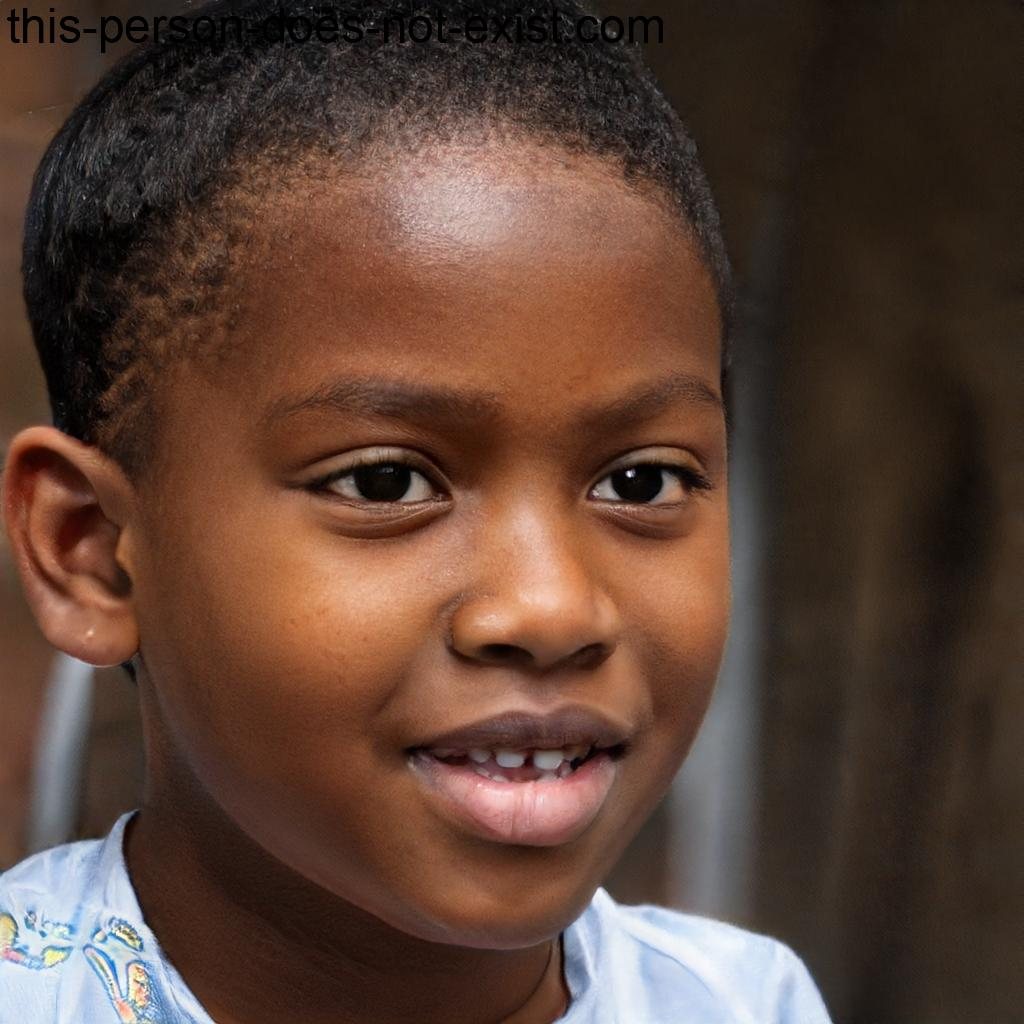
\includegraphics[width=0.5\textwidth]{this_person_does_not_exist.jpeg}
    \caption{Bild von der Webseite \href{https://this-person-does-not-exist.com}{this-person-does-not-exist.com}.}
    \label{fig:this_person_does_not_exist}
\end{figure}
Manche Bilder kann man mit Hilfe der Tipps welche unten bei der Webseite stehen noch von echten Bildern unterscheiden. Bei so vielen geht es jedoch schon nicht mehr. Dies schockte mich. Ein solches Bild kann man für 15\$ von ihnen abkaufen, was nicht viel ist wenn man bedenkt, dass man damit mehrere tausend Leute hineinlegen kann und um Spendengeld betrügen kann.
\subsection{Fazit}

Auch hier komme ich zur Schlussfolgerung, dass der ethische Aspekt im Umgang mit KI erneut bei dem Menschen liegt. Jedoch finde ich nun, dass es nicht nur noch an dem Ersteller liegt und wie stark er das Ganze einschränkt sonder, auch wie der Nutzer das Ganze nutzt.
Also all das Deepfakezeug muss ja nicht unbedingt negativ genutzt werden, es kann auch in einem lustigen Sinn verwendet werden, z.B. seine Freunde "never gonna let you down" singen zu lassen.
Auch spielt es meiner Meinung nun mehr eine Rolle was der Nutzer denn überhaupt möchte, denn nur das wird vom Ersteller erstellt.
\newpage
\section{Bedroht KI Jobs?}
Ja, in der Schweiz sind schon 60\% der Jobs von KI beinflusst. Also um einiges mehr als die Hälfte vermutlich auch mehr als Sie erwartet haben. Besonders sind jedoch folgende Jobs und Berufsgruppen:
\begin{itemize}
    \item Buchhalter/-innen
    \item Mathematiker/-innen
    \item Programmierer/-innen
    \item Kund(/-innen)support
    \item Büro und Administartion
    \item Transportwesen
    \item Zusteller/-innen
    \item Lebensmittelproduktion
\end{itemize}
Jedoch werden auch neue Jobs geschaffen werden, man teilt die neuen Jobs in folgende 3 Kategorien auf:
\begin{itemize}
    \item Trainer/-innen
    \item Erhalter/-innen
    \item Erklärer/-innen
\end{itemize}
Dabei sind Trainer/-innen hauptsächlich für die Entwicklung und Trainierung der Software zuständig. Sie müssen also schauen, dass alles funktioniert wie es soll.
Erhalter/-innen sollen für das Gleichgewicht zwischen der Einhaltung der finanziellen Zielen und der Performance der KI zu überwachen und auch zu erhalten.
Und was müssen die Erklärer/-innen machen? Die Erklärer/-innen müssen die Entscheidungen der KI's einordnen und bewerten.\citep{bedrohte-jobs-kununu}
\\
Ich selbst bin hier ein wenig unsicher was ich von der ganzen Sache halten soll. Zum einen sehe ich den  gewaltigen Fortschritt welcher KI uns bringt, zum anderen habe ich jedoch immernoch das Gefühl,
dass KI uns etwas weg nimmt und ich meine nicht nur Jobs. Ich finde, dass es uns so langsam das ganze Denken abnimmt und so wirklich befürworten kann ich dies nicht. Abgesehen davon denke ich das KI weniger Jobs schafft als das sie wegnimmt.
\\
\\
\subsection{Fazit}
Ich bleibe nach wie vor, dass KI eingeschränkt benutztbar sein soll. Aufjeden Fall nicht so offen wie es jetzt ist. Auch denke ich, dass es eine neue Art von verifizierung notwendig ist um sicher zu stellen das etwas von den echten Medien kommt.Auch bin ich nun zum Entgültigen Schluss gekommen, dass man das Thema Ethik bei einer KI nicht wirklich eine eiszeit auf den Menschen schieben darf.

\newpage
\section{Fazit}
Um zum Fazit zu kommen nenne ich euch nochmals meine Hauptfrage:
\\
Wird KI für den Menschen gefährlich?
\\
Und ja ich denke KI wird für den Menschen gefährlich, dies liegt einfach an den vielen vielen Möglichkeiten die es nun gibt.
Wenn sich das in dieser Geschwindigkeit weiterentwickelt, dann kann man bald gar niemandem mehr glauben. Selbst ofizielle Platformen/Kanäle wie SRF werden Probleme haben da auch sie von irgendwo ihre Informationen her haben müssen.
Im schlimmsten Fall würde sogar die Demokratie verloren gehen, da man nicht mal politisch sich informieren kann und daher auch nicht wirklich sagen kann für was man politisch stimmt.
Auch wird man aufpassen müssen, dass nicht plötzlich die eigene Stimme oder Videos mit dem eigenen Gesicht irgendwo auf kuriosen Webseiten zu finden sind. KI wird auch in der Kriegspolitik gewaltigen Einfluss haben.
Man kann wortwörtlich sagen, dass ein neues Zeitalter kommt. Ob gut oder schlecht hängt jedoch vom Menschen ab und wie er die neuen Möglichkeiten nutzen wird. Denn mit KI kann auch ganz viel positives entwickelt werden. Natürlich bringt dieses Jobsverlust mit sich, es wird aber auch ganz neue Arbeitsplätze mit sich bringen.
Aktuell ist alles noch ein wenig schwammig und ich denke wir sollen den kleinen aber extrem starken Helfer nutzen solange es noch so einfach möglich ist.
Hoffen wir auf das Beste.
